\documentclass[conference]{IEEEtran}
\usepackage{amsmath,amssymb}
\usepackage{graphicx}
\usepackage{booktabs}
\usepackage{multirow}
\usepackage{cite}
\usepackage{url}
\usepackage[hidelinks]{hyperref}
\usepackage{xcolor}
\newcommand{\pp}{\,pp}
\newcommand{\cond}[1]{\textsc{#1}}

\begin{document}

\title{What Makes a Virtual ISA Programmable by AI Agents?\\
A Controlled Study of Agent-Facing Interfaces to StableHLO}

% Single-blind review: author names and affiliations appear on the submission.
\author{\IEEEauthorblockN{\{Author Name(s)\}}
\IEEEauthorblockA{\{Affiliation(s)\}\\ \{email\}}}

\maketitle

\begin{abstract}
AI coding agents increasingly write and repair programs for compiler intermediate representations, yet benchmarks score the agent rather than the \emph{interface} the virtual ISA exposes to it. We hold one IR (StableHLO), one pinned verifier and executor, one task suite and the agent loop fixed, and vary only how semantic documentation reaches the agent: none, syntax-only, natural-language prose, a structured JSON contract containing the same canonical facts, and on-demand retrieval of those facts through a tool. Over 114 held-out tasks (38 templates) with independent numerical oracles, three GPT-4.1 snapshots and 2{,}052 pre-registered trials, (1)~any documentation is the dominant lever (+29 to +64\pp{} first-attempt correctness over none); (2)~the effect of a structured contract versus prose depends on model capability, from $-39.5$\pp{} for the smallest model to $+2.6$\pp{} (not significant) for the largest; and (3)~on-demand introspection underperforms upfront delivery by up to 62\pp{}, because the strongest agent never called the tool and, when forced to, retrieved operation-local facts but often missed the cross-cutting encoding rule. Of 1{,}158 failed first attempts, 1{,}157 were rejected statically; agent-facing VISA design is therefore first a problem of making well-formedness learnable. We release the harness, fact inventory, tasks, and trial logs.
\end{abstract}

\section{Introduction}
A virtual ISA earns its keep by decoupling programs from rapidly changing hardware: front ends target the virtual layer and back ends absorb the churn~\cite{lattner2004llvm,lattner2021mlir}. Increasingly, the ``front end'' is an AI agent that writes, repairs and optimizes code at the virtual layer. This adds a design dimension that ISA designers have not traditionally optimized: \emph{how the ISA is presented to a non-human programmer}. Existing benchmarks score models on producing GPU kernels~\cite{ouyang2025kernelbench,li2025tritonbench,guan2026tritongym}, LLVM IR optimizations~\cite{yang2026cirbench}, or kernels for unfamiliar accelerator ISAs~\cite{nie2026kernelcraft}. They answer ``how good is the agent?'' for a given interface. We ask the complementary question: for a fixed agent and a fixed IR, \emph{which properties of the agent-facing interface change whether the agent writes correct programs?}

We study StableHLO~\cite{stablehlospec}, a versioned, specification-backed MLIR dialect~\cite{lattner2021mlir} that serves as a portability layer between ML frameworks and compilers. Our manipulation is controlled at the level of individual facts. We authored a canonical inventory of 77 facts, anchored to clauses of the pinned specification. Each fact has two renderings, a natural-language sentence and a formal predicate. Treatments differ only in which facts are delivered and how (\S\ref{sec:design}). The study was pre-registered before the evaluation split was run; one exploratory condition added mid-run is reported as post-hoc.

\textbf{Contributions.} (i)~A controlled methodology, with harness, for varying agent-facing ISA documentation while holding IR, toolchain, tasks and agent loop fixed. (ii)~A 152-task StableHLO suite with independent numpy oracles, validated end-to-end against reference solutions and by mutation testing. (iii)~Pre-registered evidence from 2{,}052 trials, plus 342 post-hoc trials, about which interface properties matter, and a failure anatomy showing where agents break. (iv)~Concrete design implications for agent-facing virtual ISAs (\S\ref{sec:implications}).

\section{Related Work}
KernelBench~\cite{ouyang2025kernelbench} and TritonBench~\cite{li2025tritonbench} evaluate LLM generation of efficient GPU kernels from PyTorch-level references; TritonGym~\cite{guan2026tritongym} adds an agentic orchestration layer with function-call tools to separate model ability from workflow design. CIRBench~\cite{yang2026cirbench} evaluates LLMs on analyzing, repairing and optimizing LLVM IR with verifier, equivalence and performance checks. KernelCraft~\cite{nie2026kernelcraft} benchmarks agents writing low-level kernels for emerging accelerators with new ISAs, using tool feedback. All of these vary the model or the target and treat documentation and tooling as part of a fixed setup. To our knowledge, none isolates the \emph{representation and access mode} of the ISA's semantic documentation as the independent variable while holding the IR, the tasks and the agent fixed. That is our contribution, not a new leaderboard.

\section{Study Design}\label{sec:design}
\subsection{Fixed IR, toolchain and agent loop}
Programs are StableHLO modules with a single \texttt{@main}. We parse and verify them with the MLIR/StableHLO bindings in jaxlib 0.11.2 (StableHLO 1.20.0) and execute them on XLA:CPU in a sandboxed subprocess with a 60\,s timeout and an operation allow-list (no \texttt{custom\_call} or foreign dialects). The task fixes the signature exactly; a mismatched \texttt{@main} type is a failure. The agent receives a system prompt, the documentation (if any), and the task. It replies with one program; failures are returned verbatim (verifier diagnostic, or the first mismatching oracle element), allowing up to two repairs. The documentation stays in context during repairs, and in the interactive conditions the tool remains available. Budgets: 6~tool calls, 12~model calls and 2{,}048 output tokens per call. Each trial is a fresh conversation at temperature~0, run once per task and condition, in seeded random order.

\subsection{Canonical facts and interface treatments}
The inventory has 77 facts over 18 operation groups (20~syntax, 13~type, 26~shape, 18~semantics). Each fact carries an ID, a source anchor (spec section and constraint label, e.g.\ \texttt{broadcast\_in\_dim (C5)}), an \texttt{nl} sentence, and a \texttt{formal} predicate in spec notation. For example, BID.SHP.3 reads ``Operand dimension $d$ must either have size 1 or have the same size as result dimension \texttt{broadcast\_dimensions[d]}'' (prose) and $\forall d\colon \textit{dim}(\textit{operand},d){=}1 \lor \textit{dim}(\textit{operand},d){=}\textit{dim}(\textit{result},\textit{bd}[d])$ (structured). A task's fact set is the cross-cutting \texttt{module} facts (program structure, types, attribute encoding, no implicit broadcasting) plus the facts of the operations the task names as relevant. All 22 code examples in the inventory verify with the pinned toolchain. Table~\ref{tab:conds} lists the treatments. Every condition, including \cond{None}, receives the identical task statement, signature and list of relevant operations, so knowing \emph{which} operation to use is never part of the manipulation.

\begin{table}[t]
\caption{Interface treatments. Tokens: mean documentation length (o200k) over 152 tasks.}
\label{tab:conds}
\centering\footnotesize
\setlength{\tabcolsep}{3pt}
\begin{tabular}{@{}llllr@{}}
\toprule
& Condition & Facts & Rendering & Tok. \\
\midrule
-- & \cond{None} & none & -- & 0 \\
A & \cond{Minimal} & syntax & prose & 340 \\
N & \cond{Syntax-only str.} & syntax & JSON & 371 \\
B & \cond{Prose} & all & prose, no IDs & 615 \\
C & \cond{Structured} & all & JSON + IDs & 811 \\
D & \cond{Interactive} & on demand & JSON via tool & -- \\
D$^\ast$ & \cond{Forced} (post-hoc) & as D & tool call required & -- \\
\bottomrule
\end{tabular}
\end{table}

An automated audit checks every task's B/C pair. It verifies identical fact-ID sequences, that each fact's \texttt{nl} occurs verbatim in B and its \texttt{formal} in C, and that no fact ID leaks into B; a perturbed renderer fails it (unit-tested). The \cond{Interactive} tool \texttt{get\_facts(operation, category)} returns exactly the C rendering for the requested slice. It is restricted to the task's operation groups, so D has the same \emph{available} facts as B and C; we log the facts actually retrieved. N is a negative control: it changes format while carrying only syntax facts.

\subsection{Tasks and independent oracles}
We wrote 38 parametric templates covering broadcasting, reductions, \texttt{dot\_general} contractions, layout (transpose/reshape/reverse), slicing/padding/concatenation, masking and indexing (iota/compare/select, \texttt{dynamic\_slice}), element-wise operations, type conversion, and composites (softmax, L2 normalization, pairwise distance). Each template is instantiated four times with seeded, mutually distinct dimension sizes. Instance~0 is the development split, used only for harness debugging. Instances~1--3 are the frozen evaluation split: 114 tasks in 38 clusters. Each task is specified mathematically (e.g.\ ``$\mathit{out}[c,a,b]=x[a,b,c]$''). Its oracle is a numpy reference that never inspects StableHLO, evaluated on three held-out input cases that include semantic traps: all-negative rows for max-reductions, exact zeros for strict comparisons, and out-of-range starts for \texttt{dynamic\_slice} clamping. Comparison requires exact shape and dtype, exact equality for integers and booleans, and $\mathrm{rtol}{=}10^{-4}$ for f32. \textbf{Validation:} all 152 hand-written reference solutions pass parse, verify, execute and oracle. Single-point mutations of the evaluation references produced 326 mutants; 181 were rejected statically, and the oracle rejected 132 of the 145 that executed. We inspected all 13 survivors and each is semantically equivalent to its reference (e.g.\ softmax shift invariance, a reordered reduction axis list).

\subsection{Models and statistical plan}
We used three dated OpenAI snapshots spanning a capability range within one model family: \texttt{gpt-4.1-nano/-mini/-2025-04-14} (total API cost about \$6.80). A local open-weights model (Qwen2.5-7B-Instruct) solved 0 of 12 development trials, never called the tool, and was dropped before the evaluation split, as the frozen protocol records. The primary endpoint is \emph{first-attempt semantic correctness}: verified, executed and matching the oracle on all cases. The primary contrast is C$-$B. We pre-specified five paired contrasts (Table~\ref{tab:contrasts}) and report, per model, the mean paired difference with a 95\% template-cluster bootstrap CI (10k resamples; instances of one template are not independent) and exact McNemar tests on task-level discordant pairs, Holm-corrected within each model and outcome. Family-level results and D$^\ast$ are exploratory.

\section{Results}
All 2{,}052 pre-registered trials completed (114 per cell), with no exclusions. Fig.~\ref{fig:conds} and Table~\ref{tab:main} give per-condition correctness; Table~\ref{tab:contrasts} gives the contrasts.

\begin{figure*}[t]
\centering
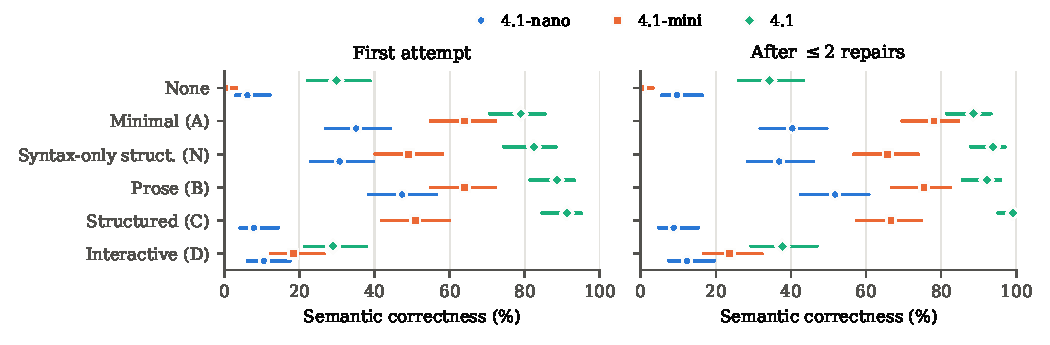
\includegraphics[width=\textwidth]{figures/fig_conditions.pdf}
\caption{Semantic correctness by interface condition (114 held-out tasks per point; 95\% Wilson intervals). Left: first attempt (primary endpoint). Right: after up to two verifier/oracle-guided repairs.}
\label{fig:conds}
\end{figure*}

\begin{table}[t]
\caption{Semantic correctness (\%) at first attempt (1st) and after $\le$2 repairs (rep.), $n{=}114$ per cell.}
\label{tab:main}
\centering\small
\setlength{\tabcolsep}{3.5pt}
\begin{tabular}{lrrrrrr}
\toprule
& \multicolumn{2}{c}{4.1-nano} & \multicolumn{2}{c}{4.1-mini} & \multicolumn{2}{c}{4.1} \\
Condition & 1st & rep. & 1st & rep. & 1st & rep. \\
\midrule
None & 6.1 & 9.6 & 0.0 & 0.0 & 29.8 & 34.2 \\
Minimal (A) & 35.1 & 40.4 & 64.0 & 78.1 & 78.9 & 88.6 \\
Syntax-only struct. (N) & 30.7 & 36.8 & 49.1 & 65.8 & 82.5 & 93.9 \\
Prose (B) & 47.4 & 51.8 & 64.0 & 75.4 & 88.6 & 92.1 \\
Structured (C) & 7.9 & 8.8 & 50.9 & 66.7 & 91.2 & 99.1 \\
Interactive (D) & 10.5 & 12.3 & 18.4 & 23.7 & 28.9 & 37.7 \\
\bottomrule
\end{tabular}
\end{table}

\begin{table}[t]
\caption{Pre-specified paired contrasts, first attempt. disc.\ = tasks solved only by the first / only by the second condition; Holm over the five contrasts per model.}
\label{tab:contrasts}
\centering\scriptsize
\setlength{\tabcolsep}{2.5pt}
\begin{tabular}{llrrrr}
\toprule
Model & Contrast & $\Delta$ (pp) & 95\% CI (cluster) & disc. & $p_\text{Holm}$ \\
\midrule
4.1-nano & Structured -- Prose & -39.5 & [-52.6, -27.2] & 0/45 & $<$0.001 \\
 & Interactive -- Structured & +2.6 & [-3.5, +9.6] & 7/4 & 0.719 \\
 & Prose -- Minimal & +12.3 & [+1.8, +22.8] & 19/5 & 0.020 \\
 & Minimal -- None & +28.9 & [+15.8, +43.0] & 34/1 & $<$0.001 \\
 & Syntax-only struct. -- Minimal & -4.4 & [-14.0, +6.1] & 7/12 & 0.719 \\
\midrule
4.1-mini & Structured -- Prose & -13.2 & [-25.4, -1.7] & 5/20 & 0.008 \\
 & Interactive -- Structured & -32.5 & [-46.5, -19.3] & 1/38 & $<$0.001 \\
 & Prose -- Minimal & +0.0 & [-8.8, +7.9] & 9/9 & 1.000 \\
 & Minimal -- None & +64.0 & [+50.0, +77.2] & 73/0 & $<$0.001 \\
 & Syntax-only struct. -- Minimal & -14.9 & [-26.3, -4.4] & 5/22 & 0.005 \\
\midrule
4.1 & Structured -- Prose & +2.6 & [-7.0, +12.3] & 8/5 & 0.848 \\
 & Interactive -- Structured & -62.3 & [-76.3, -47.4] & 0/71 & $<$0.001 \\
 & Prose -- Minimal & +9.6 & [+2.6, +19.3] & 11/0 & 0.003 \\
 & Minimal -- None & +49.1 & [+31.6, +65.8] & 59/3 & $<$0.001 \\
 & Syntax-only struct. -- Minimal & +3.5 & [-6.1, +14.0] & 9/5 & 0.848 \\
\bottomrule
\end{tabular}
\end{table}

\textbf{F1: Documentation is the dominant lever; its absence is catastrophic.} Without documentation, gpt-4.1-mini solved 0 of 114 tasks and gpt-4.1 solved 29.8\%. Syntax facts alone (A) add $+28.9$, $+64.0$ and $+49.1$\pp{} (all Holm $p<0.001$). Without documentation, failures are almost entirely malformed assembly (for gpt-4.1, 76 of its 80 failures): models produce plausible but invalid pretty-printed forms, legacy attribute encodings, or operations from other dialects. Adding the semantic and shape facts on top of syntax (B$-$A) helps less and less uniformly: $+12.3$\pp{} for nano, $0.0$ for mini, and $+9.6$\pp{} for gpt-4.1, where B solved 11 tasks that A missed and A solved none that B missed.

\textbf{F2: Structured versus prose interacts with capability.} The primary contrast C$-$B is $-39.5$\pp{} [$-52.6$, $-27.2$] for nano (45 vs.\ 0 discordant tasks), $-13.2$\pp{} [$-25.4$, $-1.7$] for mini, and $+2.6$\pp{} [$-7.0$, $+12.3$] for gpt-4.1 (not significant). After repairs, gpt-4.1 with the structured contract reaches 99.1\% (C$-$B $+7.0$\pp{}, Holm $p=0.023$). The small model's collapse under C is mainly an instantiation failure. Its attribute-encoding errors rise from 15 (B) to 43 (C), and 37 of those 43 programs write bracketed lists (\texttt{dimensions = [..]}) instead of instantiating the documented \texttt{array<i64: d0, ...>} schema. The negative control points the same way. Changing only the format of syntax facts (N$-$A) costs mini $-14.9$\pp{} ($p_\text{Holm}=0.005$) and is not significant for the other two models. A machine-readable contract is therefore not free: it pays off only when the agent can reliably instantiate schemas into concrete syntax.

\textbf{F3: On-demand introspection underperforms upfront delivery, for two separable reasons.} D$-$C is $-32.5$\pp{} for mini and $-62.3$\pp{} for gpt-4.1, and not significant for nano, whose C rate is already near the floor. \emph{Uptake:} nano and mini called the tool in 100\% and 97\% of trials (2.4 and 2.9 calls, retrieving 63\% and 78\% of available facts), but gpt-4.1 \emph{never} called it (0 of 114) and wrote programs from its priors. \emph{Scope:} in the post-hoc D$^\ast$ condition, which forces a tool call on the first turn, gpt-4.1 reached 50.0\% [41, 59]. That is $+21.1$\pp{} over D but still $-41.2$\pp{} below C, despite 3.4 calls per trial and about 2.5$\times$ C's input tokens. Forced retrieval did not change mini or nano. The agent's queries were operation-local (mostly \texttt{syntax}). In the 49 forced trials where it also fetched the cross-cutting \texttt{module} facts, including the integer-list attribute encoding rule, it was correct 87.8\% of the time, close to C's 91.2\%. In the other 65 trials it was correct 21.5\% of the time, and 62\% of those trials failed on attribute encoding, typically the legacy \texttt{dense<[..]>} form. This comparison is observational, since the agent chose what to retrieve, but it identifies where on-demand interfaces leak: agents do not know which facts they are missing.

\textbf{F4: Agents fail at well-formedness, not numerics.} Of 1{,}158 failed first attempts, 1{,}157 were rejected by the parser or verifier. Across all 5{,}097 attempts in the study, 1{,}147 programs executed, and only 4 of them produced wrong values. A post-hoc, diagnostic-based taxonomy of the failed first attempts gives: invalid assembly syntax 48\%, attribute encoding 20\%, malformed literals 14\%, shape/type verifier errors 13\%, unknown operations 4\%. Repairs add 0--16.7\pp{} (Fig.~\ref{fig:conds}, right), so verifier diagnostics are a usable but limited feedback channel.

\section{Implications for Agent-Facing VISAs}\label{sec:implications}
\textbf{Ship a normative, version-pinned surface syntax with concrete instances.} The most common specific error was drift toward an older attribute encoding that the current verifier rejects. Agents carry stale priors about evolving IRs, so the interface must state the current concrete form, not only the abstract grammar.
\textbf{Cross-cutting facts must not depend on retrieval.} Encoding conventions, type syntax and the absence of implicit broadcasting apply to every operation. Introspection APIs should return them with every operation-level answer, or the ISA should include them in every interaction.
\textbf{Structure is capability-dependent.} Formal contracts helped the strongest model after repair and hurt weaker ones. Pairing each schema with a worked instance is a cheap hedge.
\textbf{Introspection needs uptake design.} A tool that a strong agent never calls is equivalent to no documentation. Required first retrieval, or diagnostics that point to the relevant fact IDs, are design choices that the interface, not the model, controls.

\section{Threats to Validity}
\emph{Instance vs.\ schema confound.} For syntax facts, the prose rendering carries a concrete instance (\texttt{array<i64: 1>}), while the formal rendering carries a schema (\texttt{array<i64: ...>}). C$-$B and N$-$A therefore contrast ``prose with instances'' against ``JSON with schemas'', and we cannot attribute F2 to format alone. A $2{\times}2$ follow-up (format $\times$ instantiation) is needed. \emph{Length:} C is about 31\% longer than B in tokens. \emph{Generality:} we tested one model family and one IR, at temperature~0 with one trial per cell, on synthetic tasks that are small and fully specified. Because failures are almost all static, our oracle rarely decided an outcome, so these results speak to syntactic and structural programmability more than to semantic reasoning. Validated translations of KernelBench/TritonBench tasks remain future work. \emph{Authoring:} the fact inventory and the equivalence audit were produced by the study authors with AI assistance, and the audit is necessary but not sufficient. An independent human audit of fact fidelity is pending. \emph{Post-hoc analyses:} D$^\ast$ and the failure taxonomy were defined after observing data and are labelled as such. \emph{Contamination:} our tasks are newly generated, but StableHLO syntax is public and appears in model training data.

\section{Conclusion}
Holding the IR, toolchain, tasks and agent fixed, we find that the agent-facing interface of a virtual ISA changes correctness by tens of percentage points. Documentation presence dominates. The value of structure depends on agent capability. On-demand access fails unless cross-cutting facts are delivered unconditionally and uptake is designed in. Agent-facing VISAs should be engineered as interfaces, measured with controlled experiments, and shipped with machine-checkable, version-pinned surface syntax.

\section*{Artifact Availability}
Harness, fact inventory, task generator, oracles, frozen protocol (with hashes), all trial logs and transcripts: [repository URL to be added].

\bibliographystyle{IEEEtran}
\bibliography{refs}
\end{document}
